\documentclass[12pt]{exam}
\usepackage[utf8]{inputenc}

\usepackage{amsmath,amstext,amsthm,amssymb,amsxtra}
\usepackage[top=1.5in, bottom=1.5in, left=1.25in, right=1.25in]	{geometry}
%\usepackage[normalem]{ulem}
\usepackage{txfonts} % pxfonts txfonts 
\usepackage[T1]{fontenc}
\usepackage{lmodern}
\renewcommand*\familydefault{\sfdefault}
 \usepackage{euler}   % better than the option below
\usepackage{pdfsync}
\usepackage{multicol}
\newcommand{\ci}[1]{_{ {}_{\scriptstyle #1}}}
\usepackage{graphicx}
\graphicspath{ {images/} }


\newcommand{\norm}[1]{\ensuremath{\left\|#1\right\|}}
\newcommand{\abs}[1]{\ensuremath{\left\vert#1\right\vert}}
\newcommand{\ip}[2]{\ensuremath{\left\langle#1,#2\right\rangle}}
\newcommand{\p}{\ensuremath{\partial}}
\newcommand{\pr}{\mathcal{P}}

\newcommand{\pbar}{\ensuremath{\bar{\partial}}}
\newcommand{\db}{\overline\partial}
\newcommand{\D}{\mathbb{D}}
\newcommand{\B}{\mathbb{B}}
\newcommand{\Sp}{\mathbb{S}}
\newcommand{\T}{\mathbb{T}}
\newcommand{\R}{\mathbb{R}}
\newcommand{\Z}{\mathbb{Z}}
\newcommand{\C}{\mathbb{C}}
\newcommand{\N}{\mathbb{N}}
\newcommand{\Q}{\mathbb{Q}}
\newcommand{\mQ}{\mathcal{Q}}
\newcommand{\mS}{\mathcal{S}}
\newcommand{\scrH}{\mathcal{H}}
\newcommand{\scrL}{\mathcal{L}}
\newcommand{\td}{\widetilde\Delta}
\newcommand{\pw}{\text{PW}}
\newcommand{\esup}{\text{ess.sup}}
\newcommand{\Tn}{\mathcal{T}_n}
\newcommand{\Bn}{\mathbb{B}_n}
\newcommand{\rt}{\mathcal{O}}
\newcommand{\avg}[1]{\langle #1 \rangle}
\newcommand{\one}{\mathbbm{1}}
\newcommand{\eps}{\varepsilon}
\newcommand{\grad}{\nabla}

\newcommand{\La}{\langle }
\newcommand{\Ra}{\rangle }
\newcommand{\rk}{\operatorname{rk}}
\newcommand{\card}{\operatorname{card}}
\newcommand{\ran}{\operatorname{Ran}}
\newcommand{\osc}{\operatorname{OSC}}
\newcommand{\im}{\operatorname{Im}}
\newcommand{\re}{\operatorname{Re}}
\newcommand{\tr}{\operatorname{tr}}
\newcommand{\vf}{\varphi}
\newcommand{\f}[2]{\ensuremath{\frac{#1}{#2}}}

\newcommand{\kzp}{k_z^{(p,\alpha)}}
\newcommand{\klp}{k_{\lambda_i}^{(p,\alpha)}}
\newcommand{\TTp}{\mathcal{T}_p}
\newcommand{\m}[1]{\mathcal{#1}}
\newcommand{\md}{\mathcal{D}}
\newcommand{\qan}{\abs{Q}^{\alpha/n}}
\newcommand{\sbump}[2]{[[ #1,#2 ]]}
\newcommand{\mbump}[2]{\lceil #1,#2 \rceil}
\newcommand{\cbump}[2]{\lfloor #1,#2 \rfloor}

\newcommand{\class}{Math 629 Spring 26}
\newcommand{\term}{Fall 24}
\newcommand{\examnum}{Homework \hwnum}
\newcommand{\examdate}{\duedate}
\newcommand{\timelimit}{75 Minutes}
\newcommand{\vc}[3]{\langle #1,#2,#3\rangle}
\newcommand*{\vv}[1]{\vec{\mkern0mu#1}}
\newcommand{\bv}[1]{\boldsymbol{#1}}
\newcommand{\hide}[1]{}
\newcommand{\uvec}[1]{\boldsymbol{\hat{\textbf{#1}}}}
\newcommand{\vex}[1]{\boldsymbol{{\textbf{#1}}}}

\pagestyle{head}
\firstpageheader{}{}{}
\runningheader{\class}{\examnum\ - Page \thepage\ of \numpages}{\examdate}
\runningheadrule

\makeatletter
\renewcommand*\env@matrix[1][*\c@MaxMatrixCols c]{%
  \hskip -\arraycolsep
  \let\@ifnextchar\new@ifnextchar
  \array{#1}}
\makeatother

%\printanswers
\begin{document}

\noindent
\begin{tabular*}{\textwidth}{l @{\extracolsep{\fill}} r @{\extracolsep{6pt}} l}
\textbf{\class} & \textbf{Name: Mengxiang Jiang} \\
\end{tabular*}\\
\rule[2ex]{\textwidth}{2pt}
%

 

\newcommand{\duedate}{02/02/2026 at 11:59pm}
\newcommand\hwnum{3}

Turn this assginment in on gradescope. All work must be neat and legible. Turn in 
a ``final draft''. There should be nothing scratched out and your work should flow
generally from left to right and top to bottom. 

\begin{questions}
\question
Complete the proof of the volume of the sphere (that is, assuming things balance as 
I discussed in the surface area video and given the volume of a cylinder and 
cone find the volume of a sphere via the balancing argument Archimedes gave). 
\\\\
So in the video, you showed that a scale with a cylinder on one side
and a cone and hemisphere on the other side. The scale would balance if the
cylinder had radius $2r$, height $r$, and with the center of mass of the cylinder
at $\frac{r}{2}$ from the fulcrum (deduced by symmetry since the cylinder is uniform
and lies from 0 to $r$),
while the cone and hemisphere both had radius $r$ and were at distance $2r$
from the fulcrum. Using this, we have the following equality:
\[
  V_{cyl} \times \frac{r}{2} =  V_{cone} \times 2r + V_{hem} \times 2r.
\]
We know that the volume of the cylinder is $V_{cyl} = \pi (2r)^2 \cdot r = 4\pi r^3$,
and the volume of the cone is $V_{cone} = \frac{1}{3} \pi r^2 \cdot r = \frac{1}{3} \pi r^3$.
Substituting these into the equation above, we get
\[
  2\pi r^4 = \frac{1}{3} \pi r^3 \cdot 2r + V_{hem} \times 2r.
\]
From this, we can solve for $V_{hem}$:
\[
  V_{hem} = \frac{2\pi r^4 - \frac{2}{3} \pi r^4}{2r} = \frac{(6\pi r^4 - 2\pi r^4)}{6r} = \frac{4\pi r^3}{6} = \frac{2}{3} \pi r^3.
\]
Thus, the volume of the hemisphere is $\frac{2}{3} \pi r^3$, and therefore the volume of the sphere is
\[
  V_{sph} = 2 \times V_{hem} = 2 \times \frac{2}{3} \pi r^3 = \frac{4}{3} \pi r^3.
\]

\newpage
\question 
Why does the "method of exhaustion" not work when computing the arc-length of the graph of a
function? (I don't need a very precise argument - just your best stab at why this doesn't work.)
\\\\
We can have another overestimate of the arc-length by circumscribing 
the arc by n tangent line segments at the center of the n rectangles (see figure below).
\begin{figure}[!h]
  \begin{center}
  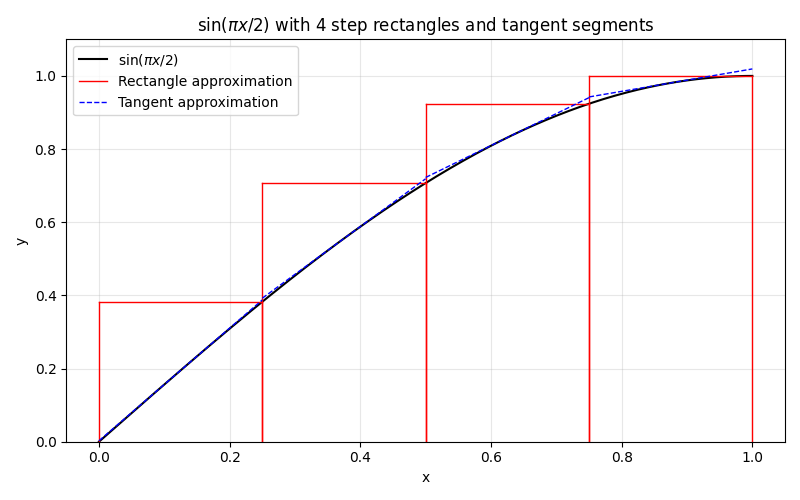
\includegraphics[width=0.6\textwidth]{arc_estimate.png}
  \caption{Estimate of arc-length}
  \end{center}
\end{figure}
If the rectangle estimate approaches the arc-length, you would expect it to
also approach the length of the tangent line segments, but as we increase n,
the difference between the two actually increases rather than decrease, indicating
the approximation error does not go to zero. Thus, this method of exhaustion
does not work for arc-length.

\newpage 
\question 
For a given circle, show that the area of the circumscribed polygons approaches the
area of the circle. 
\\\\
The argument is very similar to the one we used in class for inscribed polygons.
Instead of showing the leftover area of the circle goes to zero, 
we will show that the leftover area of the circumscribed polygon goes to zero.
We can divide the leftover area into $n$ congruent shapes near each vertex of the polygon.
This area is bounded above by the area of a triangle with base slightly less than
the side length of the polygon and height equal to the difference between the
circumradius $R$ and the inradius $r$ of the polygon. See figure below.
\begin{figure}[!h]
  \begin{center}
  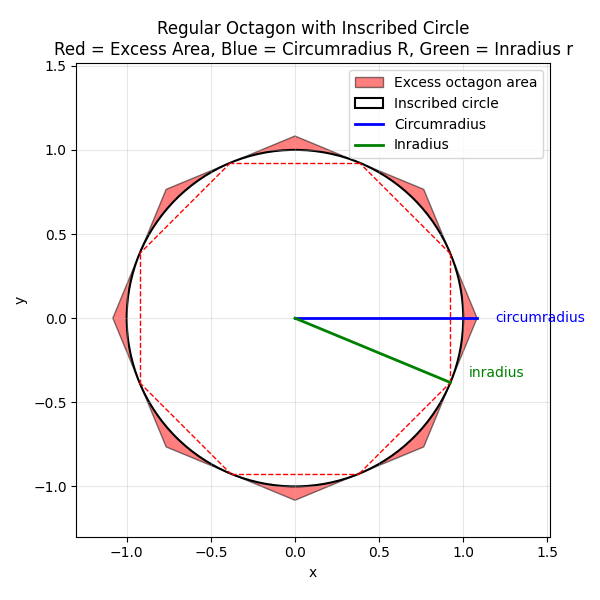
\includegraphics[width=0.6\textwidth]{circumscribed_poly.png}
  \caption{Excess area of circumscribed polygon}
  \end{center}
\end{figure}
As the number of sides of the polygon increases, the difference between the
circumradius and inradius decreases and approaches zero. Thus the area of each of these
triangles also approaches zero, which also forces the leftover area to approach zero.
Therefore, the area of the circumscribed polygon approaches the area of the circle.


\newpage 
\question 
Show that the area of a N sided regular polygon is $\frac{1}{2}a_NP_N$ where 
$a_n$ is the apothem and $P_N$ is the perimeter.
\\\\
For any regular polygon, we can divide it into $N$ congruent triangles
by drawing line segments from the center of the polygon to each vertex.
Each triangle has a base length of $\frac{P_N}{N}$ and height equal to the apothem $a_N$.
Thus, the area of each triangle is
\[
  A_{tri} = \frac{1}{2} \cdot \frac{P_N}{N} \cdot a_N.
\]
Since there are $N$ such triangles in the polygon, the total area of the polygon is
\[
  A_{poly} = N \cdot A_{tri} = N \cdot \frac{1}{2} \cdot \frac{P_N}{N} \cdot a_N = \frac{1}{2} a_N P_N.
\]
By the way, I was taught this formula as
\[
  A_{poly} = rs,
\]
where $r$ is the inradius (which is the same as the apothem for regular polygons)
and $s$ is the semiperimeter.

\end{questions}
\end{document}
